\documentclass{article}
\usepackage[utf8]{inputenc}

\usepackage[a4paper]{geometry}
\usepackage{calc}
\usepackage{float}
\usepackage{graphicx}

\usepackage{hyperref}

\usepackage{tikz}
\usetikzlibrary{arrows.meta}
\usetikzlibrary{shapes}

\setcounter{secnumdepth}{-1}

\geometry{
	left=1.5cm,
	right=2.5cm,
	top=2cm,
	bottom=4cm
}

\title{Design Paper}
\author{Giang Nguyen, Lydia Kalkbrenner, Philipp Oberwegner}

\begin{document}

\maketitle

\section{I. Issue Trend Analysis}

\begin{figure}[h]

\begin{minipage}[c]{5cm}

\beginpgfgraphicnamed{Diag-f1}
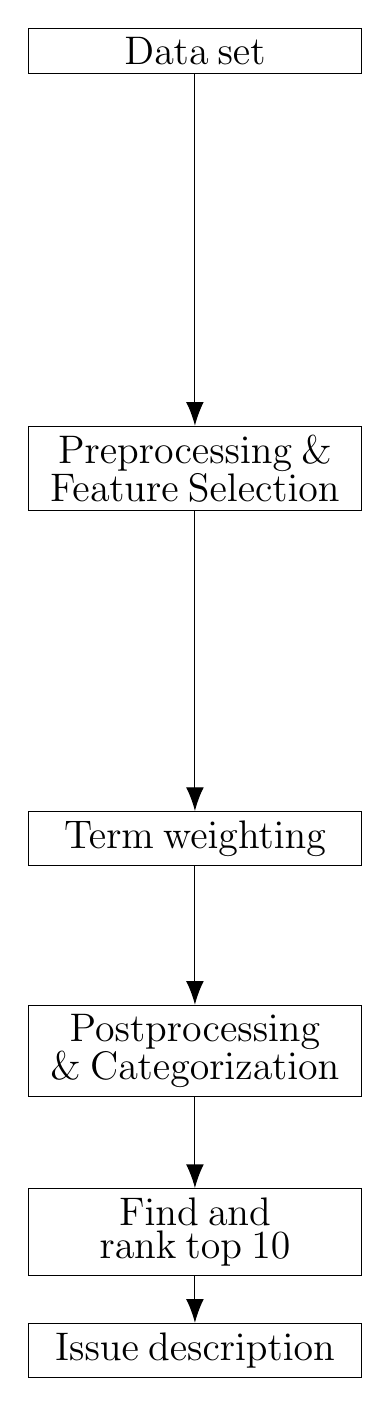
\begin{tikzpicture}
\node(A) at (0,14) [rectangle,draw=black,text width=4cm]{\Large \centerline{Data set}};
\node(B) at (0,8.7) [rectangle,draw=black,text width=4cm]{\Large \centerline{Preprocessing \&} \centerline{Feature Selection}};
\node(C) at (0,4) [rectangle,draw=black,text width=4cm]{\Large \centerline{Term weighting}};
\node(D) at (0,1.3) [rectangle,draw=black,text width=4cm]{\Large \centerline{Postprocessing} \centerline{\& Categorization}};
%\node(E) at (0,1) [rectangle,draw=black,text width=4cm]{\Large \centerline{Categorization}};
\node(F) at (0,-1) [rectangle,draw=black,text width=4cm]{\Large \centerline{Find and} \centerline{rank top 10}};
\node(G) at (0,-2.5) [rectangle,draw=black,text width=4cm]{\Large \centerline{Issue description}};
\node(Z) at (0,-3) [rectangle,text width=4cm]{};

\draw[-{Latex[length=3mm]}] (A.south -| B.north) -- (B.north);
\draw[-{Latex[length=3mm]}] (B.south -| C.north) -- (C.north);
\draw[-{Latex[length=3mm]}] (C.south -| D.north) -- (D.north);
\draw[-{Latex[length=3mm]}] (D.south -| F.north) -- (F.north);
%\draw[-{Latex[length=3mm]}] (D.south -| E.north) -- (E.north);
%\draw[-{Latex[length=3mm]}] (E.south -| F.north) -- (F.north);
\draw[-{Latex[length=3mm]}] (F.south -| G.north) -- (G.north);
\end{tikzpicture}
\endpgfgraphicnamed

\end{minipage}
\begin{minipage}[c]{\textwidth-4cm}

\large

\subsection{Problem Definition:} Given a collection of newspaper articles for three years, we were asked to find the top 10 issues for each year and rank them based on prominence and salience. Therefore we have to come up with a way to extract issues from the article collection and find a ranking method that can represent the prominence of the issues within the article collection.
After ranking the issues we have to extract a description out of the articles that are related to an issue.\\
\\
\textbf{Step I:} 
In this step we will create a bag of words for each article and apply tokenization and stemming methods. We will also compare the words to a dictionary and try to match synonyms with WordNet.
Then we will need to do some feature selection to reduce the dimension of the vector space model that we are going to create in the next step.
As we learned in the lecture, the document frequency measure is a well performing method for feature selection because it is very close to the optimal and also easy to compute, so this could be the the method of our choice.\\
\\
\textbf{Step II:} To transfer the article collection into the vector space model we want to use a more sophisticated measure for term weighting than just frequency based weighting. Because we can't estimate the performance yet, we will try different term weighting methods.\\
\\
\textbf{Step III:} In this step we will identify the issues by clustering. We make the assumption that the features that we selected occur in the same document if they belong to the same issue. We will identify classes of similar articles by running a clustering algorithm like k-means.\\
\\
\textbf{Step IV:} To determine the ranking of the identified issue we will use the number of articles that belong to one issue.\\
\\
\textbf{Step V:} For simplicity we will determine the common words between the documents of an issue for the description of an issue.

\end{minipage}

\end{figure}

\section{II. Issue Tracking}

\begin{figure}[H]

\vspace*{-6cm}

\begin{minipage}[c]{5cm}

\beginpgfgraphicnamed{Diag-f1}
\begin{tikzpicture}
\node(O) at (0,13) [rectangle,text width=4cm]{};
\node(A) at (0,6) [rectangle,draw=black,text width=4cm]{\Large \centerline{Top 10 issues}};
\node(B) at (0,1.3) [rectangle,draw=black,text width=4cm]{\Large \centerline{Pick top 2 issues}};
\node(C) at (0,-0.3) [rectangle,draw=black,text width=4cm]{\Large \centerline{Fill out} \centerline{the template}};
\node(D) at (0,-4) [rectangle,draw=black,text width=4cm]{\Large \centerline{Inter-dependent}};
\node(E) at (5,-4) [rectangle,draw=black,text width=4cm]{\Large \centerline{Independent}};
\node(F) at (0,-6) [rectangle,draw=black,text width=4cm]{\Large \centerline{Visualization:} \centerline{Flow chart}};
\node(G) at (5,-6) [rectangle,draw=black,text width=4cm]{\Large \centerline{Visualization:} \centerline{Table}};
\node(Z) at (0,-8) [rectangle,text width=4cm]{};
\draw[-{Latex[length=3mm]}] (A.south -| B.north) -- (B.north);
\draw[-{Latex[length=3mm]}] (B.south -| C.north) -- (C.north);
\draw[-{Latex[length=3mm]}] (C.south -| D.north) -- (D.north);
\draw[-{Latex[length=3mm]}] (C.south) -- (E.north);
\draw[-{Latex[length=3mm]}] (D.south -| F.north) -- (F.north);
\draw[-{Latex[length=3mm]}] (E.south -| G.north) -- (G.north);
\end{tikzpicture}
\endpgfgraphicnamed

\end{minipage}
\begin{minipage}[c]{\textwidth-4cm}

\large

\subsection{Problem Definition:} As we finished task 1, we now have top 10 issues for each year. The goal of this task is to track events associated with an issue. From top 10 issues, we will pick 2 issues for analyzing, and each issue we should identify at least 10 events. For each event, their outstanding attributes need to be extracted. There are two different types of  events:  inter-dependent  and independent events.  For each of the two chosen issues, we will identify all inter-dependent and independent events.\\

\textbf{Step I:} From top 10 issues for each year, we will pick the two most notable issues from the list of 10.\\

\textbf{Step II:} From our domain-specific knowledge about the two issues we chose, we will create a template that can be filled out by information extraction methods. We can for example extract the date and place, people or organizations involved in each event.

\end{minipage}

\end{figure}

\large

\begin{flushleft}

\vspace*{-1cm}

\textbf{Step III:} At this step, we should indicate dependence of events of an issue. We assume that inter-dependent incidents will refer to others, and to build the order of events, we could check the chronological relation amongst them. Remaining events, finally, can be group into non-dependent group of issues.\\

\centerline{}

\textbf{Step IV:} As we have two group of non-dependence and dependence, we will visualize the result in table format with non-dependent ones and flow-chart for dependent events.

\end{flushleft}

\end{document}
